\chapter{Appearance Computations}
\label{chap:appearance}

So far, we have covered the fundamental basics of the light and the rendering process to be able to comprehend the more advanced techniques practiced in computer graphics. As we have mentioned before, our primary goal is to evaluate the computational accuracy of several specific appearance sensations. Even though they are quite common in everyday life, their integration to the modern renderers is, to this date, rare. In this chapter, we discuss these phenomena individually --- their manifestations in nature, the physics behind them, and, finally, their computations in the rendering process. 

\section{Reflectance}

Reflective surfaces are a surprisingly common sighting. As the perfectly diffuse materials practically do not exist in nature, a large set of materials that surround us is considered glossy. In \autoref{sec:BRDF}, we explained the bidirectional reflectance distribution function that defines the reflective properties of a material. 

\subsection{Fresnel equations}

It is necessary to know the basics of geometry optics to be able to properly define a reflectance model. First of all, \emph{Snell's law}~\cite{pharr2016physically}

\begin{equation}
\eta_i sin\theta_i = \eta_t sin\theta_t 
\end{equation}

states that the incoming angle $\theta_i$ (angle between the surface normal and the incoming direction) times the \emph{index of refraction} of the entering medium $\eta_i$ must be equal to their transmitted counterparts. In other words, knowing the indices of refraction of the entering and the leaving media and the incoming direction, we can compute the transmitted direction.

The index of refraction (IOR) varies from material to material (e.g. IOR of glass is $\sim$1.5) and it essentially describes the ratio between the speed of light in the vacuum and the speed of light in the current medium: 

\begin{equation}
n=\frac{c}{v}
\end{equation}

, where $n$ is the IOR, $c$ is the speed of light in the vacuum and $v$ is the phase velocity of light in the current medium.

However, this gives us only the direction of the refracted light. In most cases, it is also necessary to know the ratio between the amount of reflected and the amount of refracted light. Depending on the polarization of the light (further explained in \autoref{sec:polarization}), the \emph{Fresnel equations}~\cite{pharr2016physically} take the two following forms:

\begin{align*}
r_s = \frac{\eta_t cos\theta_i - \eta_i cos\theta_t}{\eta_t cos\theta_i + \eta_i cos\theta_t}\\
r_p = \frac{\eta_i cos\theta_i - \eta_t cos\theta_t}{\eta_i cos\theta_i + \eta_t cos\theta_t} 
\end{align*}

From these, we can compute the \emph{Fresnel reflectance} for an unpolarized light:
\begin{equation}
F_r=\frac{1}{2}(r_s^2 + r_p^2)
\end{equation}

According to the energy conservation law, the transmitted energy is equal to $1-F_r$.

Note that the previous computations describe only \emph{dielectrics} --- materials that do not conduct electricity and are capable of transmitting light, such as glass, water, diamond, etc. The second large group, \emph{conductors}, consists of all materials with opaque surfaces, such as metals. Conductors also transmit light, however, due to their physical properties, it is quickly absorbed. There also exists a third group called \emph{semiconductors} which are rarely considered in the physically-based rendering and therefore we skip them. A comparison between a dielectric and a conductor is shown in \autoref{fig:compare_dielectric_conductor}.

\begin{figure}[h]
	\centering
	\begin{tabular}{cc}
		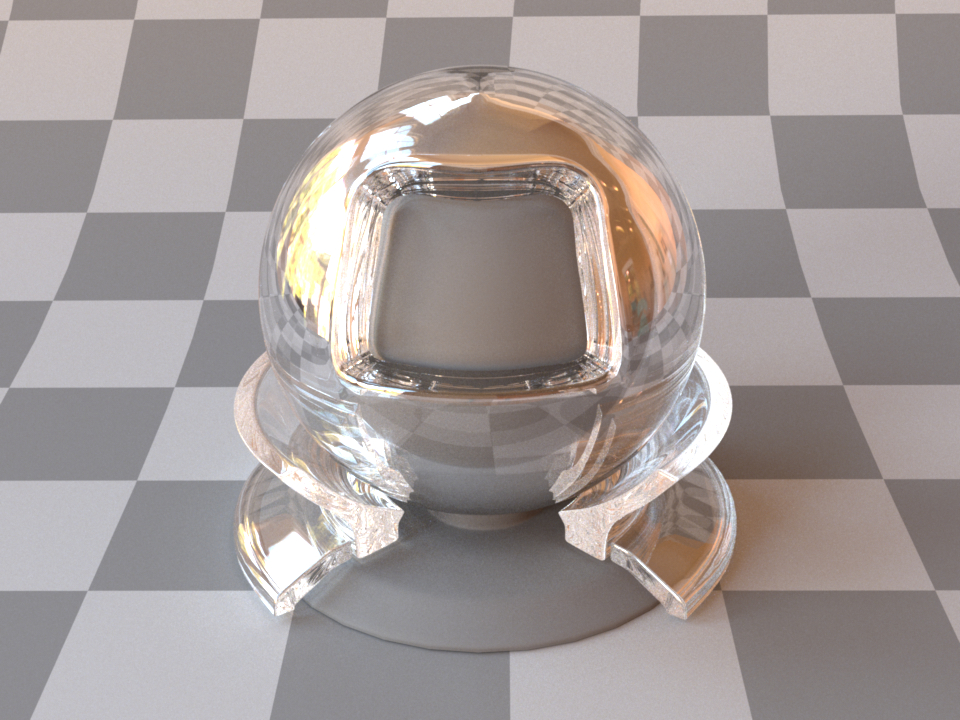
\includegraphics[width=.4\linewidth]{img/dielectric_diamond.jpg}
		&
		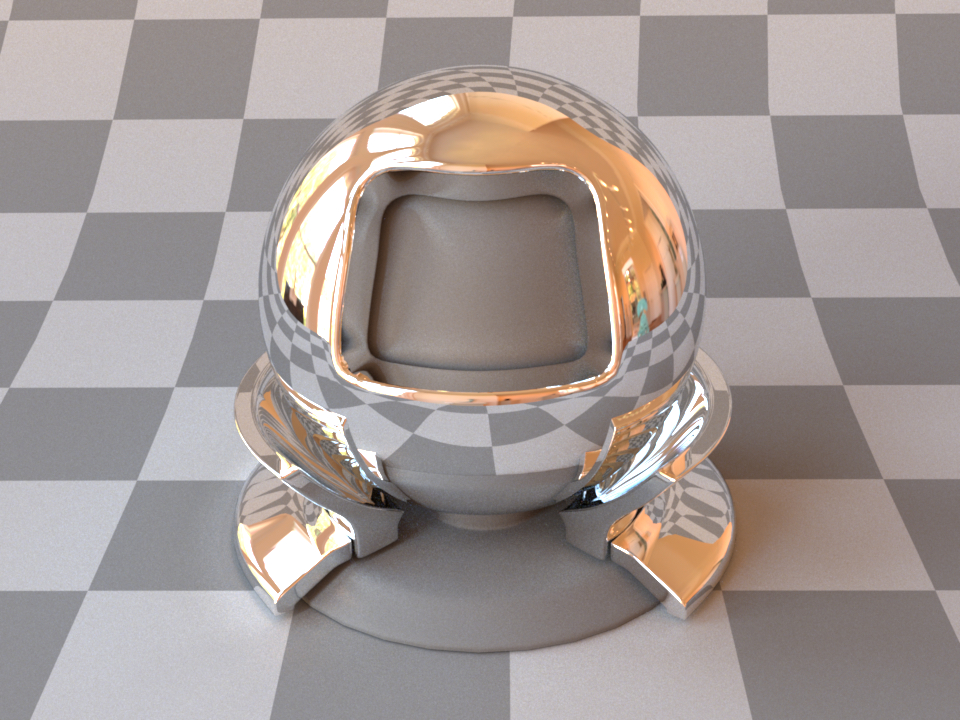
\includegraphics[width=.4\linewidth]{img/conductor_aluminium.jpg}
	\end{tabular}
	\caption{A preview of a dielectric (diamond, left) a conductor (aluminum, right) rendered in Mitsuba2~\cite{mitsubaWeb}}
	\label{fig:compare_dielectric_conductor}
\end{figure}

While this is a simple matter of computing the Fresnel equations, the practice is usually more complicated. Most of the commonly seen materials are at least slightly rough, either on purpose or due to the manufacturing errors.

\subsection{Microfacet theory}
To describe rough surfaces, the \emph{microfacet theory} was introduced by \citet{cook1982reflectance}.

The main idea is that a rough surface consists of \emph{microfacets} -- a collection of very small surfaces distributed statistically throughout the whole underlying \emph{macrosurface}. The aggregate behavior of the computed values for each of these microfacets determines the final scattering. An example of such distribution is shown in \autoref{fig:microfacets}.

\begin{figure}[h]
	\centering
	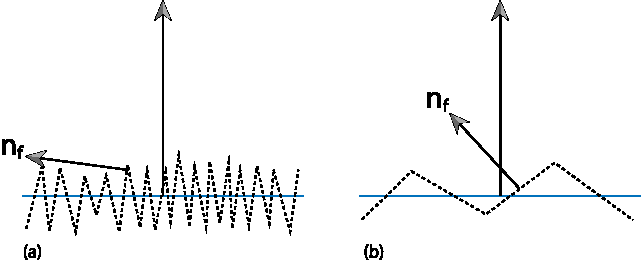
\includegraphics[width=.8\linewidth]{img/microfacets.pdf}
	\caption{A demonstration of a very rough (left) and a relatively smooth (right) microfacet distribution~\cite{pharr2016physically}}
	\label{fig:microfacets}
\end{figure}

As the microfacet computations are local, we need to consider the possibility that they might obscure each other. Three main aspects are accounted for:
\begin{description}
	\item[Masking] Microfacet is not visible from the viewer
	\item[Shadowing] Microfacet is not reachable from the light source
	\item[Interrecflection] Bounces between the microfacets
\end{description}

Many variations to the Cook-Torrance model have been developed, such as its predecessor Torrance-Sparrow~\cite{Torrance1967TheoryFO} model or Oren-Nayar~\cite{oren1994generalization} model for diffuse reflectance.

In this thesis, we focus on the microfacet distribution functions, as they are ultimately the deciding factor of the rough surface look. A nice comparison of the three commonly used microfacet distributions --- \emph{Phong}, \emph{Beckmann}, and \emph{GGX} --- along with their distribution functions, masking functions and sampling equations, can be found in the article by \citet{walter2007microfacet}. As the exact formulations of these methods are not a necessity for this thesis, we provide only a brief overview for each of them. We also provide a comparison between the GGX model and the Beckmann model in
\autoref{fig:ggx_beckmann}.

\paragraph{Phong}

Even though the Phong distribution is purely empirical (not physically based), it is still a quite popular choice for the microfacet distribution, as it is simple to implement and provides sufficient results.

\paragraph{Beckmann}

The Beckmann distribution~\cite{beckmann1987scattering} is already physically based and for a long time has been considered the best solution to the rough surfaces, as it is based on the Gaussian roughness. However, with the parameters set appropriately, it still provides results very similar to the Phong distribution.

\paragraph{GGX}

The GGX distribution~\cite{walter2007microfacet} was introduced as an improvement of the Beckmann's solution for some cases. It maintains stronger tails, thus has better shadowing, and it is based on the measured data of the real rough materials.

\begin{figure}[h]
	\centering
	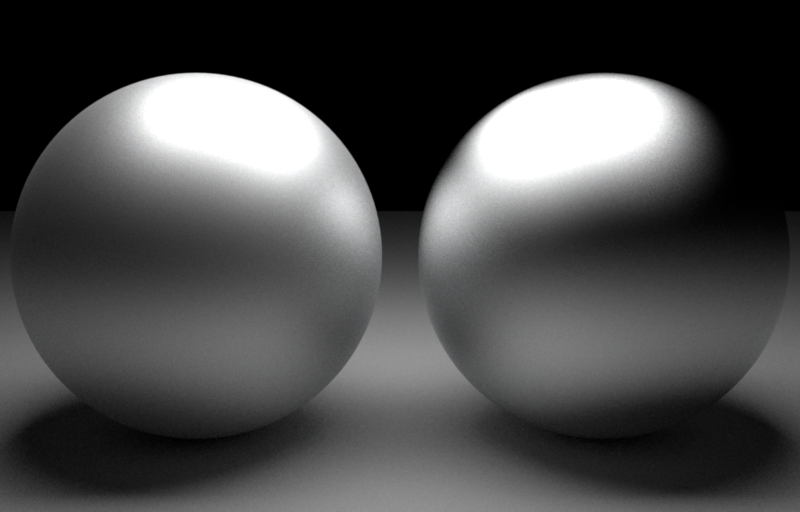
\includegraphics[width=.8\linewidth]{img/ggx_beckmann.png}
	\caption{A rough aluminum sphere with the GGX distribution (left) compared to its Beckmann equivalent (right) rendered in Mitsuba2}
	\label{fig:ggx_beckmann}
\end{figure}

\section{Polarization}
\label{sec:polarization}

Similarly to all kinds of electromagnetic radiation, the light also propagates through space as a wave. The oscillation direction of this wave neither defines nor modifies the color of the light. However, it makes the light behave differently upon interaction with certain materials. \autoref{fig:oscillation} explains the different directions of a wave.

\begin{figure}[h]
	\centering
	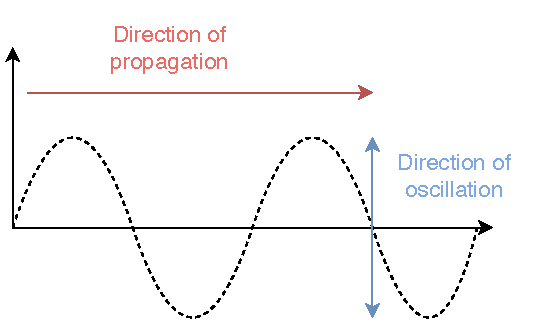
\includegraphics[width=.6\linewidth]{img/oscillation.pdf}
	\caption{Demonstration of the direction of oscillation and the direction of propagation}
	\label{fig:oscillation}
\end{figure}

In the light's natural state (sun, common light bulb), the directions of its oscillation are arbitrary --- such light is called \emph{unpolarized}. The \emph{polarized} light maintains a restricted direction of oscillation and it is a result of a \emph{polarization} process. Note that the light is often only partially polarized, as the restriction of the direction does not have to be perfect and allows some variations.

In reality, each photon is polarized --- by default, it keeps the same restricted direction of oscillation until surface interaction. The photons of polarized light are all polarized in the same manner while the photons of unpolarized light are polarized randomly. 

Depending on the shape of their electric fields, we distinguish three types of polarization, which are demonstrated in \autoref{fig:polar_types}.

\begin{figure}[h]
	\centering
	
\includegraphics[width=.7\linewidth]{img/polar_types.png}
	\caption[polar types]{An illustrative demonstration of the different types of polarization \footnotemark}
	\label{fig:polar_types}
\end{figure}
\footnotetext{\url{http://hyperphysics.phy-astr.gsu.edu/hbase/phyopt/polclas.html}}

To create polarized light, a dielectric object may be placed in the direction of propagation of unpolarized light. Due to the optical properties of the dielectrics, the reflected and the transmitted light will be polarized proportionally to the angle of the incidence. The angle at which the reflected light is perfectly polarized is called \emph{Brewster's angle}~\cite{brewster1815laws}. It is computed by the following formula:

\begin{equation}
\theta=arctan(\frac{n_2}{n_1})
\end{equation}
, where $n_1$ is the IOR of the exterior and $n_2$ of the transmitted medium.

In the simplest case of a reflection from a dielectric plane, we distinguish two types of linearly polarized light depending on the relative orientation of their polarization to the incident plane. The reflected light is called \emph{p-polarized}, as its oscillation is parallel to the plane of incidence. The transmitted light is called \emph{s-polarized}, as its oscillation is perpendicular to the plane of incidence. Both are shown in \autoref{fig:brewster}.

\begin{figure}[h]
	\centering
	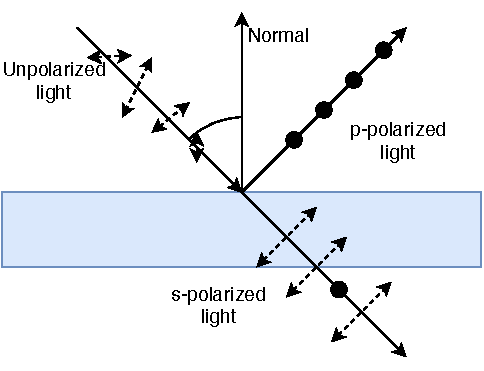
\includegraphics[width=.7\linewidth]{img/brewster.pdf}
	\caption{Perfectly p-polarized reflected light and partially s-polarized refracted light due to an interaction with a dielectric interface under Brewster's angle}
	\label{fig:brewster}
\end{figure}


The principle of Brewster's angle is commonly used in a material called the \emph{linear polarizer}. As the name suggests, it polarizes the light, restricting its direction of oscillation according to the properties of the polarizer. If the light that passes through the polarizer is of the opposite (perpendicular) direction to the polarizer's transmission orientation, it will not let it through and no light will be visible. \autoref{fig:polarizer} illustrates the effects of a polarizer.

\begin{figure}[h]
	\centering
	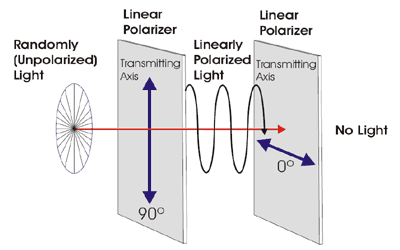
\includegraphics[width=.6\linewidth]{img/polarizer.png}
	\caption[nikon]{Unpolarized light passes through a vertical polarizer $\rightarrow$ linearly vertically polarized light passes through a horizontal polarizer $\rightarrow$ no light\footnotemark}
	\label{fig:polarizer}
\end{figure}
\footnotetext{\url{www.apioptics.com/about-api/resources/visible-light-linear-polarizer/}}

This property is frequently incorporated in sunglasses or camera filters to reduce the glare of the sun reflected from a horizontal surface. The reflected p-polarized light goes through a polarizer with a perpendicularly oriented transmission axis, which consequently eliminates the incoming light. The effect of a polarizing filter is shown in \autoref{fig:polarizer_nikon}.

\begin{figure}[h]
	\centering
	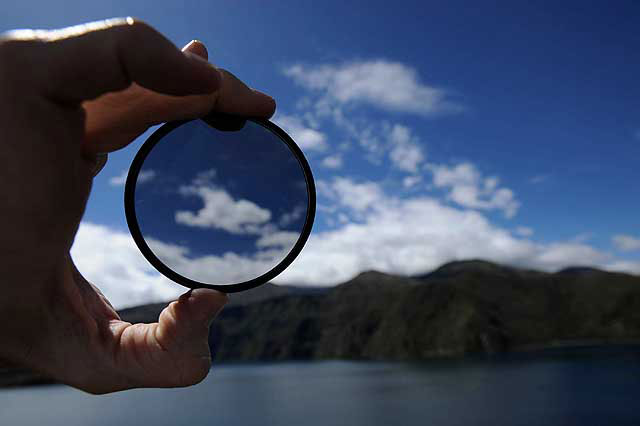
\includegraphics[width=.7\linewidth]{img/polarizer_nikon.jpg}
	\caption[nikon]{Polarizing filter by Nikon\footnotemark}
	\label{fig:polarizer_nikon}
\end{figure}
\footnotetext{\url{https://www.nikonusa.com/en/learn-and-explore/a/tips-and-techniques/polarizing-filters-add-pow-to-pictures.html}}

The information about the polarization we cover in this section is sufficient for the purposes of this thesis so we do not need to go into further detail. If the reader wishes to learn more, please refer to scientific literature, for example, the \emph{Polarized light in optics and spectroscopy}~\cite{kliger2012polarized}

\subsection{Polarization in rendering}
The integration of polarization in the rendering process is quite rare. Only a few scenarios display the effects of polarization and one must implement quite complex behavior of the radiation waves to spectral rendering. However, Mitsuba2 and ART fully track the polarization state of light when needed. The implementation covered by this section is already in Mitsuba2~\cite{mitsubaWeb}.

The polarization state is represented by the \emph{Stokes vector} --- a 4-dimensional quantity that parameterizes the elliptical shape of the light's electric field for each wavelength separately. The information stored in the Stokes vectors is explained in \autoref{fig:stokes}.

\renewcommand\thesubfigure{\arabic{subfigure}}
\begin{figure}
	\centering
	\begin{tabular}{cc}
		\begin{subfigure}
			{0.4\textwidth}\centering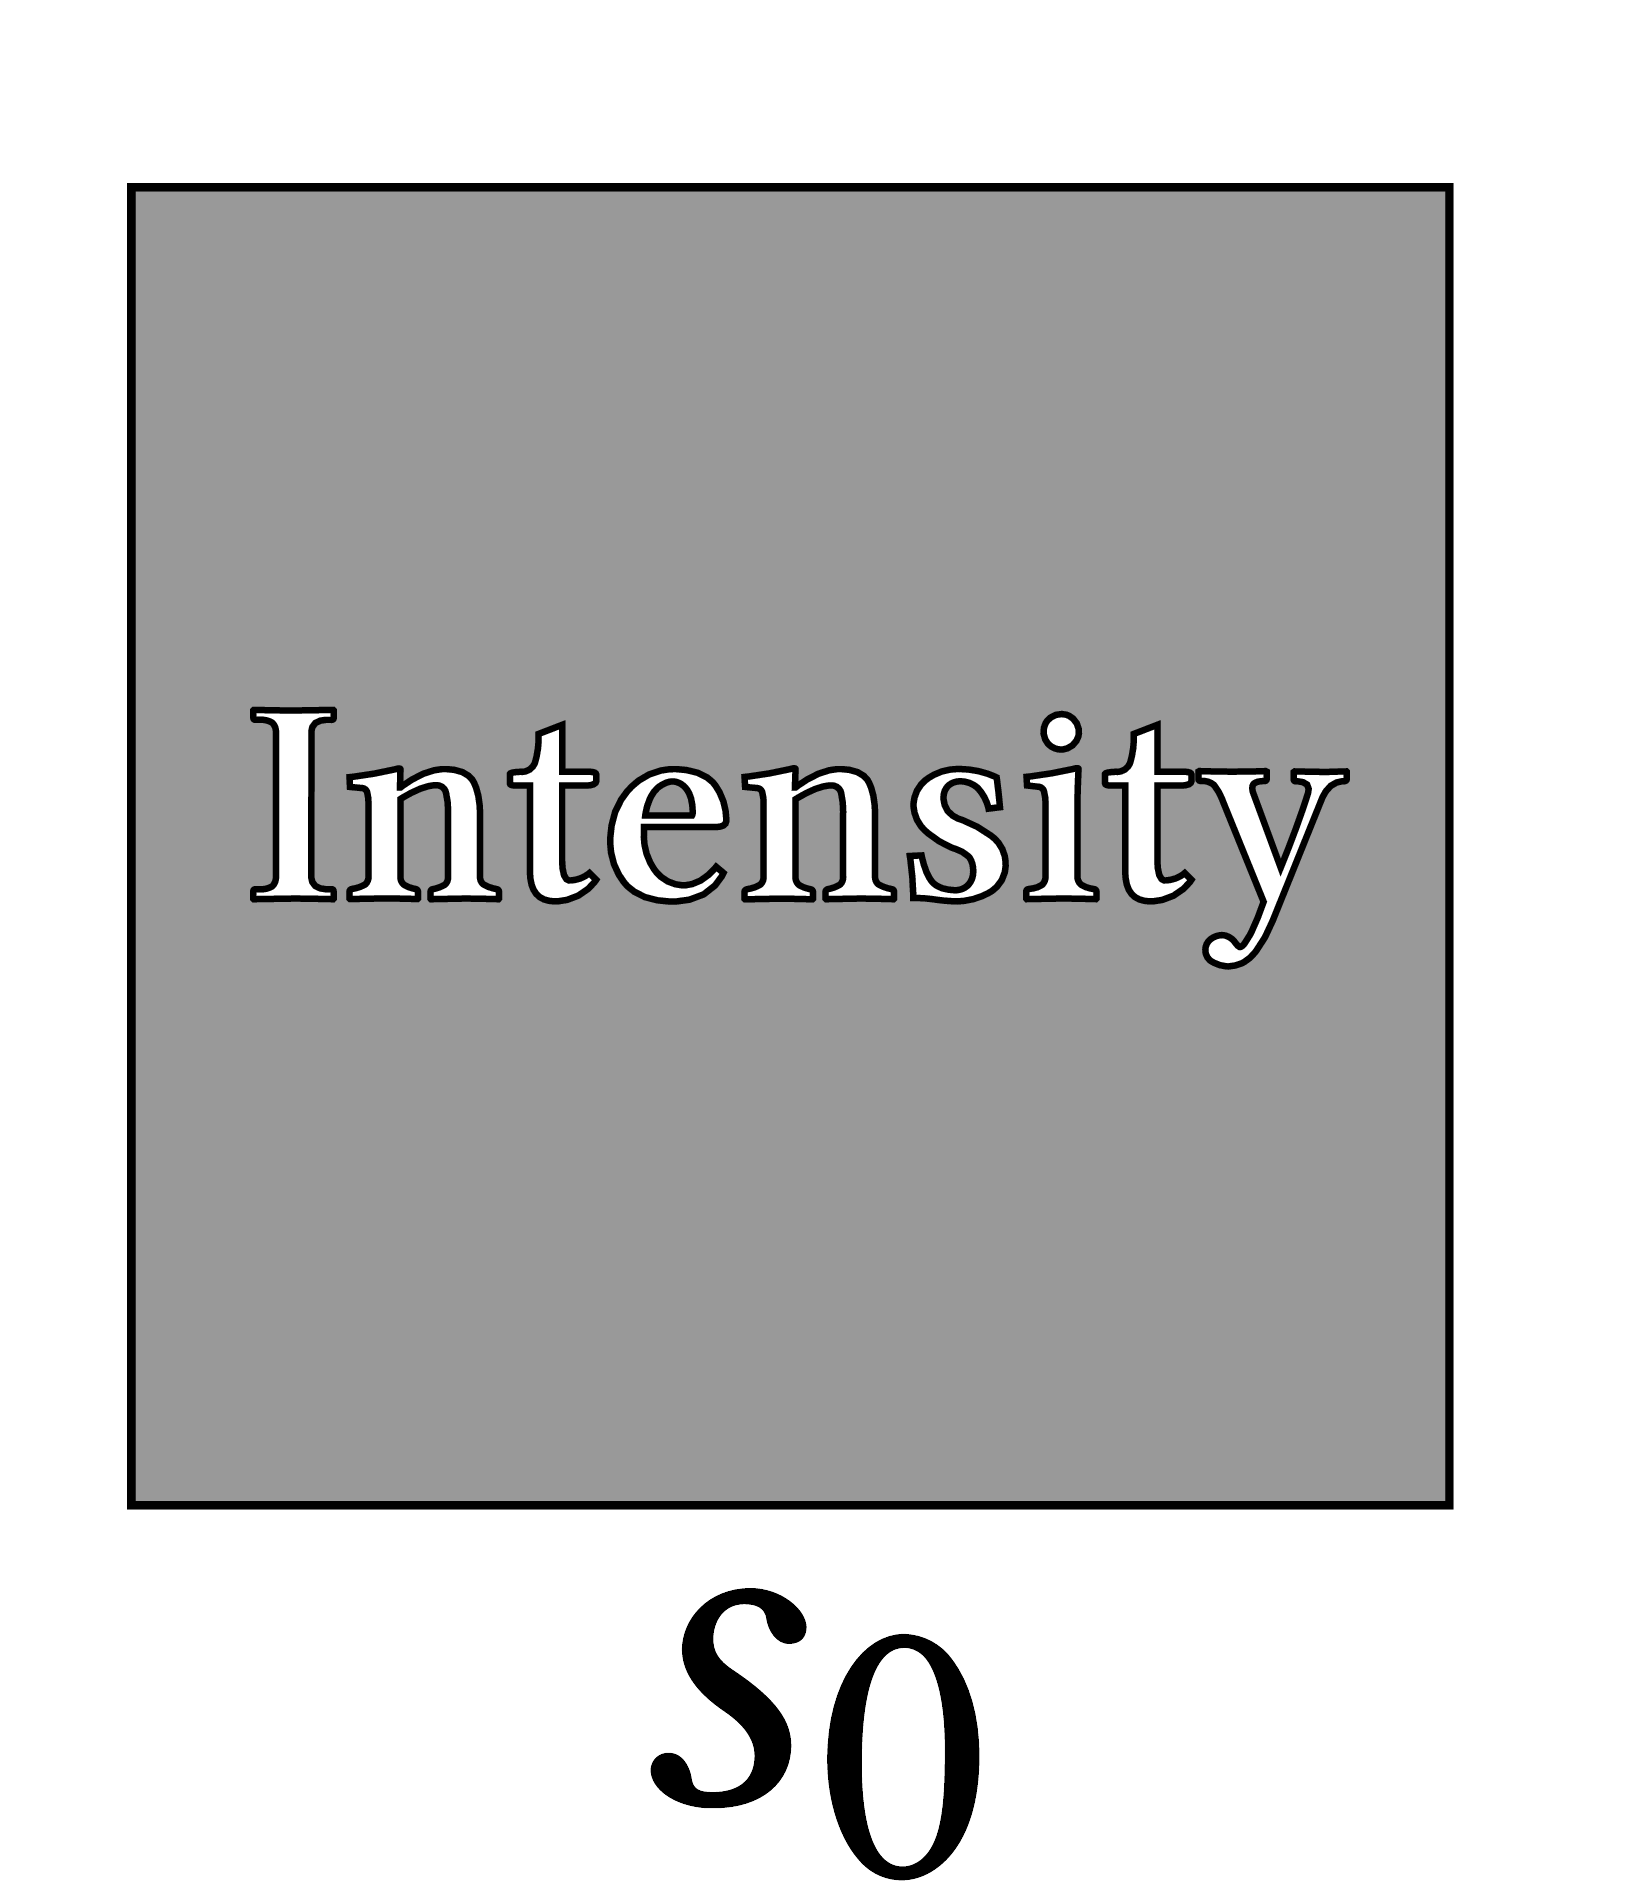
\includegraphics[width=\linewidth]{img/stokes1.png}
			\caption{Radiance - no polarization}
		\end{subfigure}
		&
		\begin{subfigure}
			{0.4\textwidth}\centering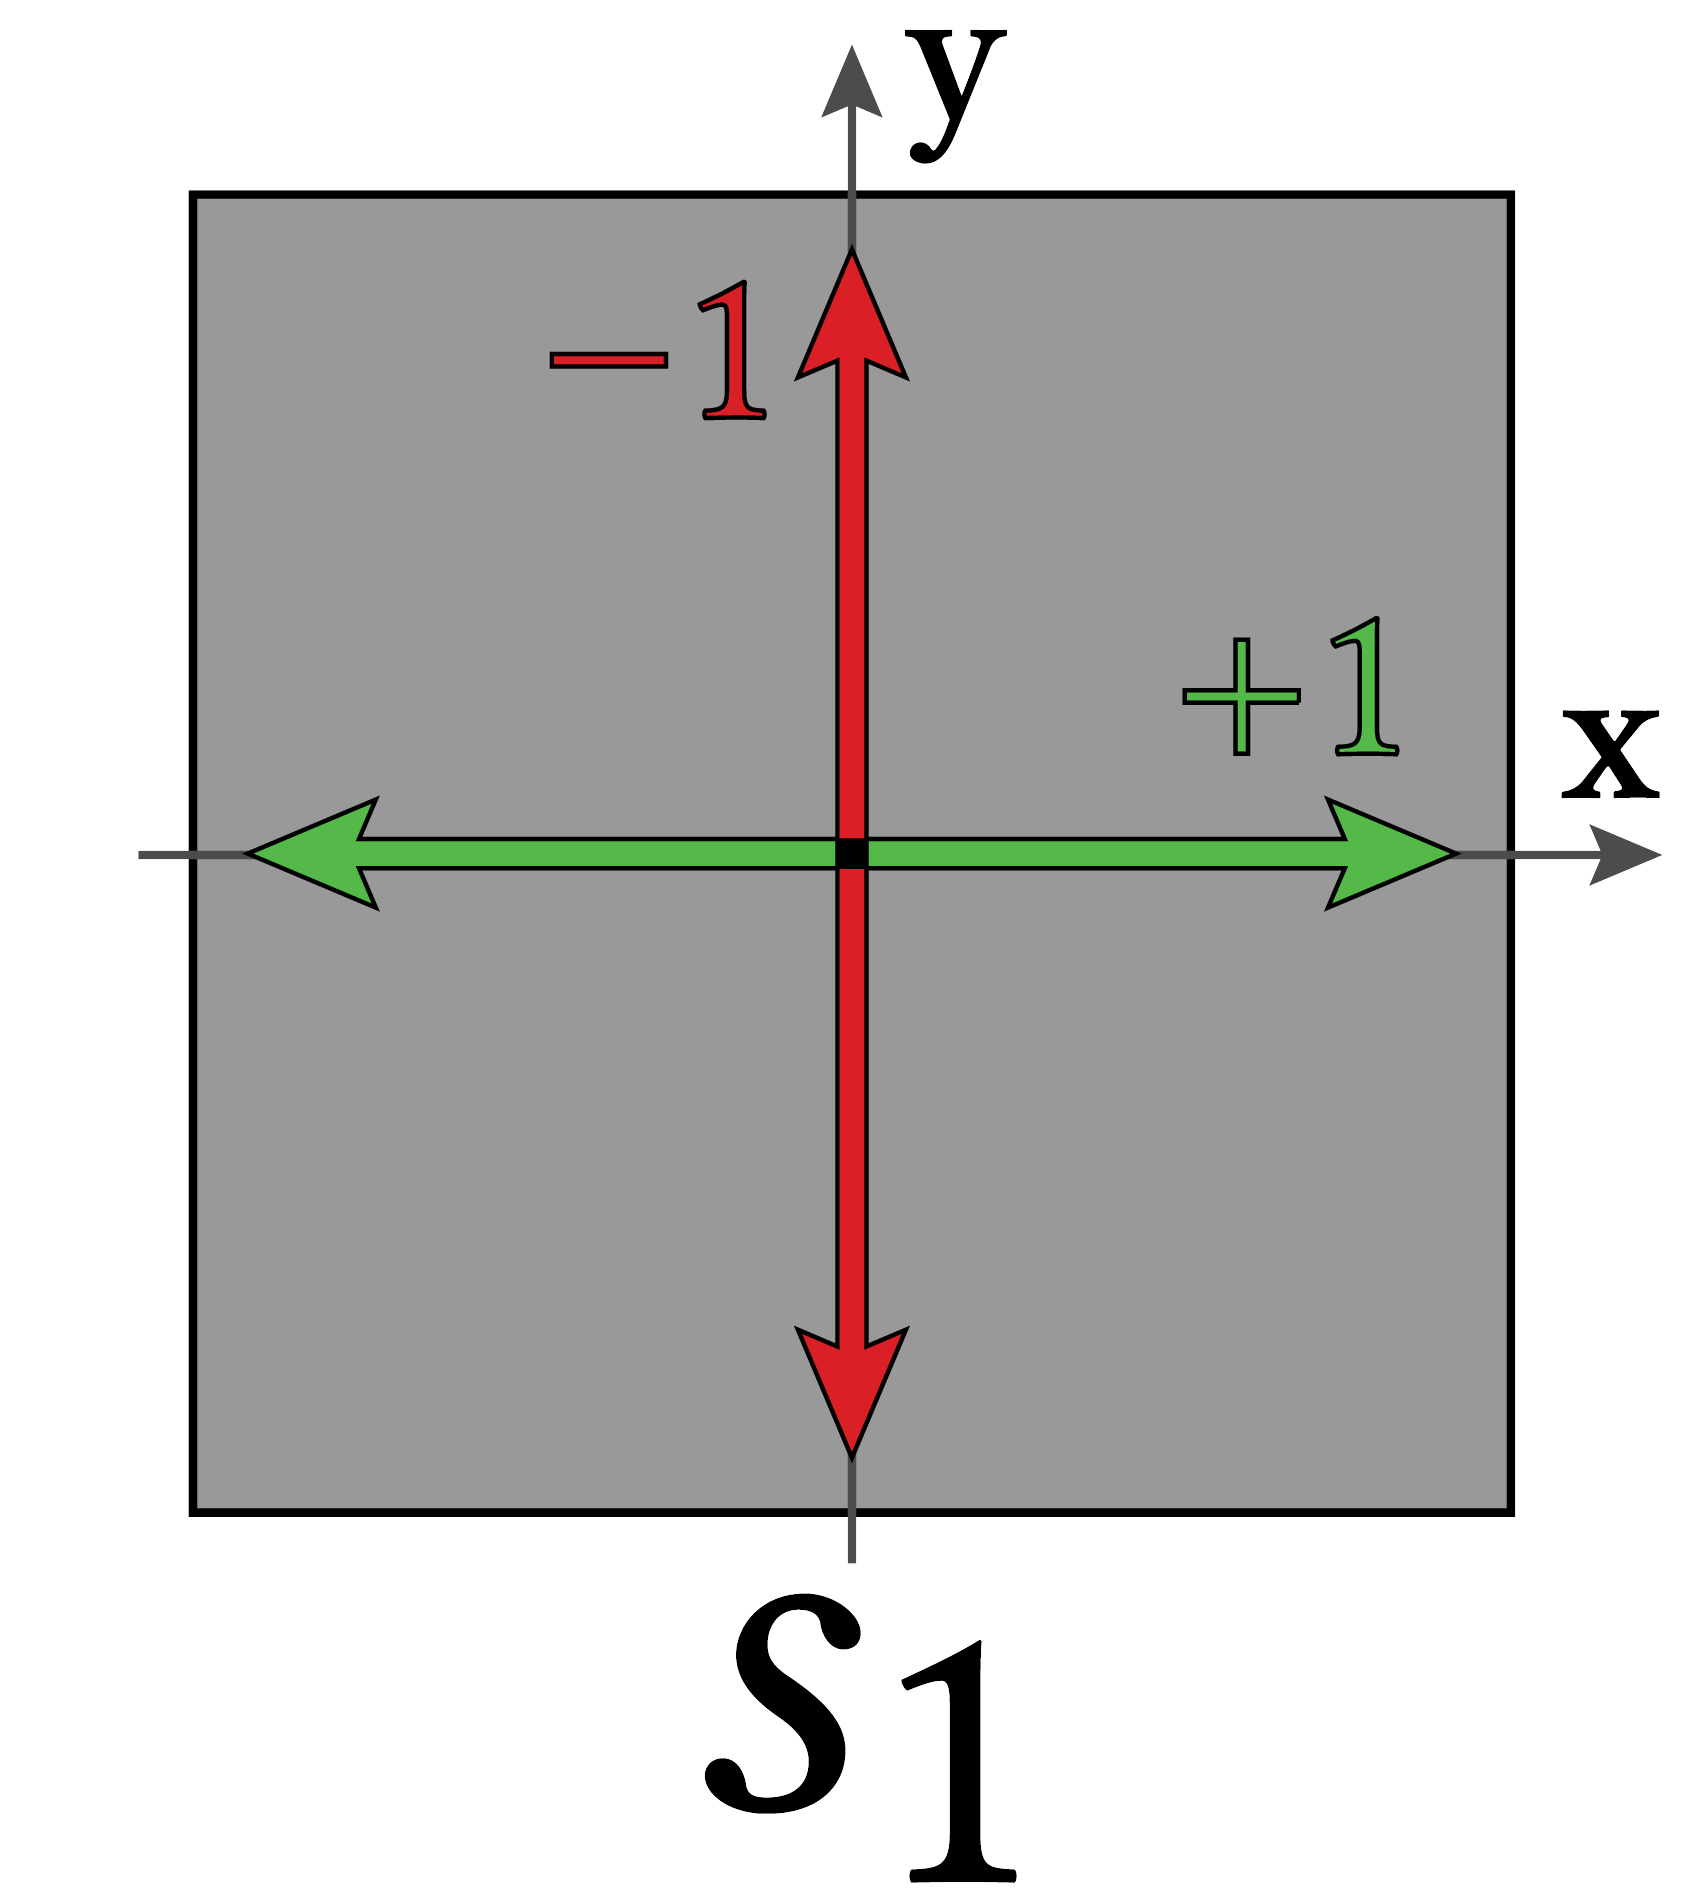
\includegraphics[width=\linewidth]{img/stokes2.png}
			\caption{Horizontal vs. vertical polarization}
		\end{subfigure} \\
		\begin{subfigure}
			{0.4\textwidth}\centering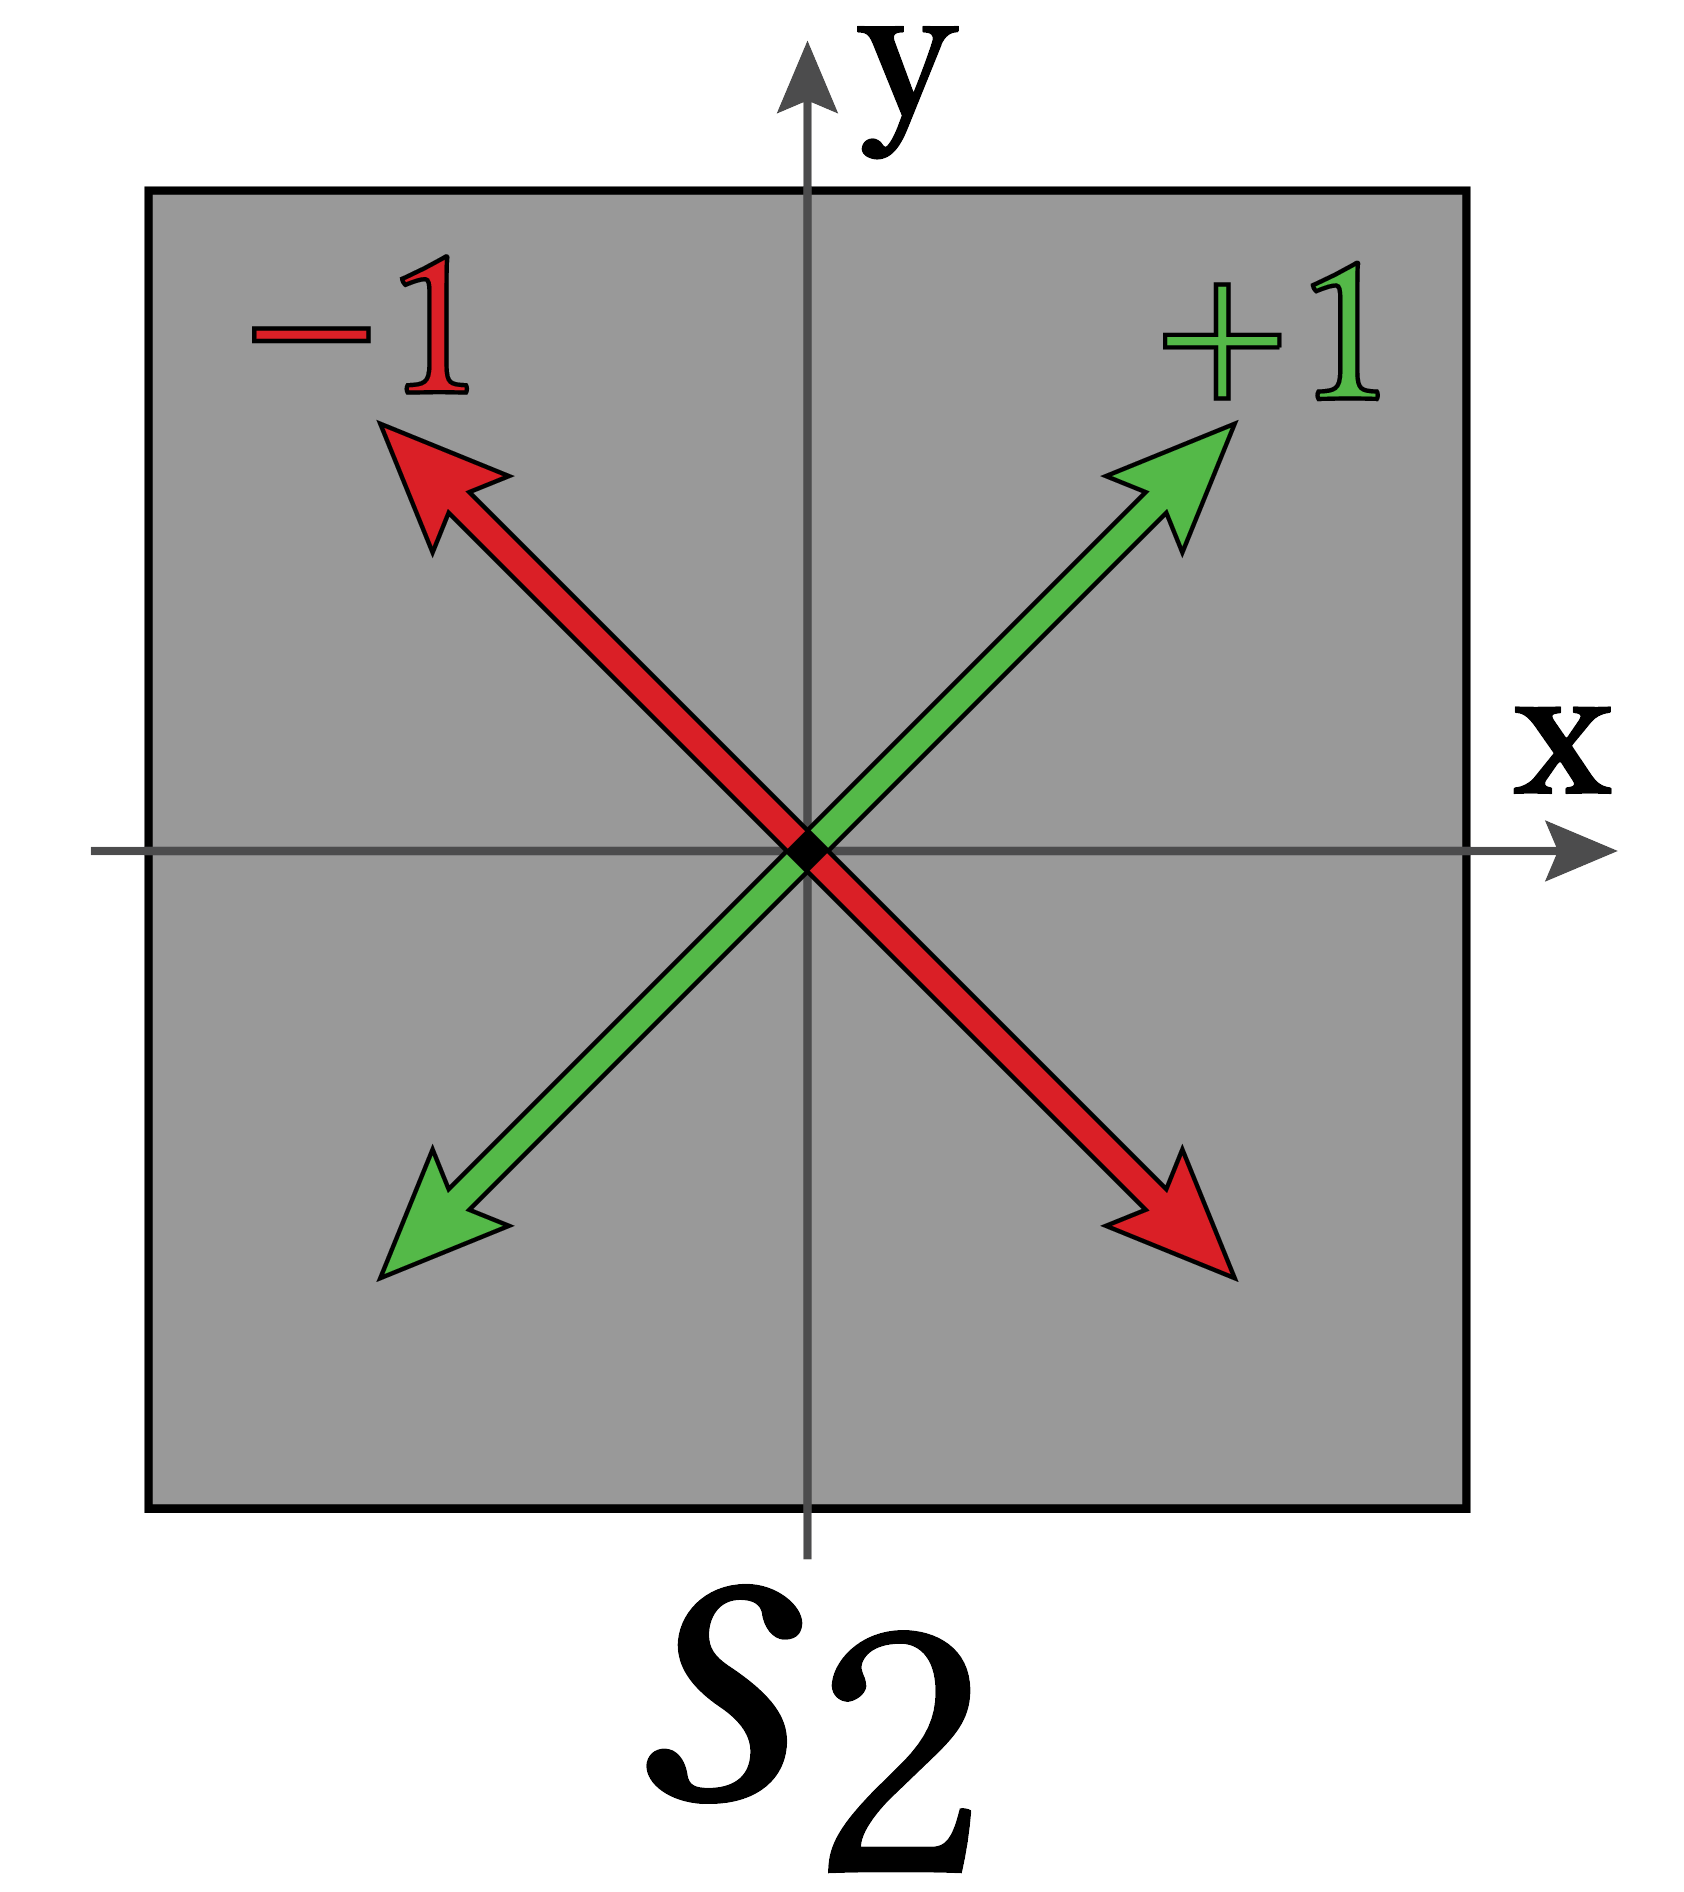
\includegraphics[width=\linewidth]{img/stokes3.png}
			\caption{Diagonal polarization}
		\end{subfigure} 
		&
		\begin{subfigure}
			{0.4\textwidth}\centering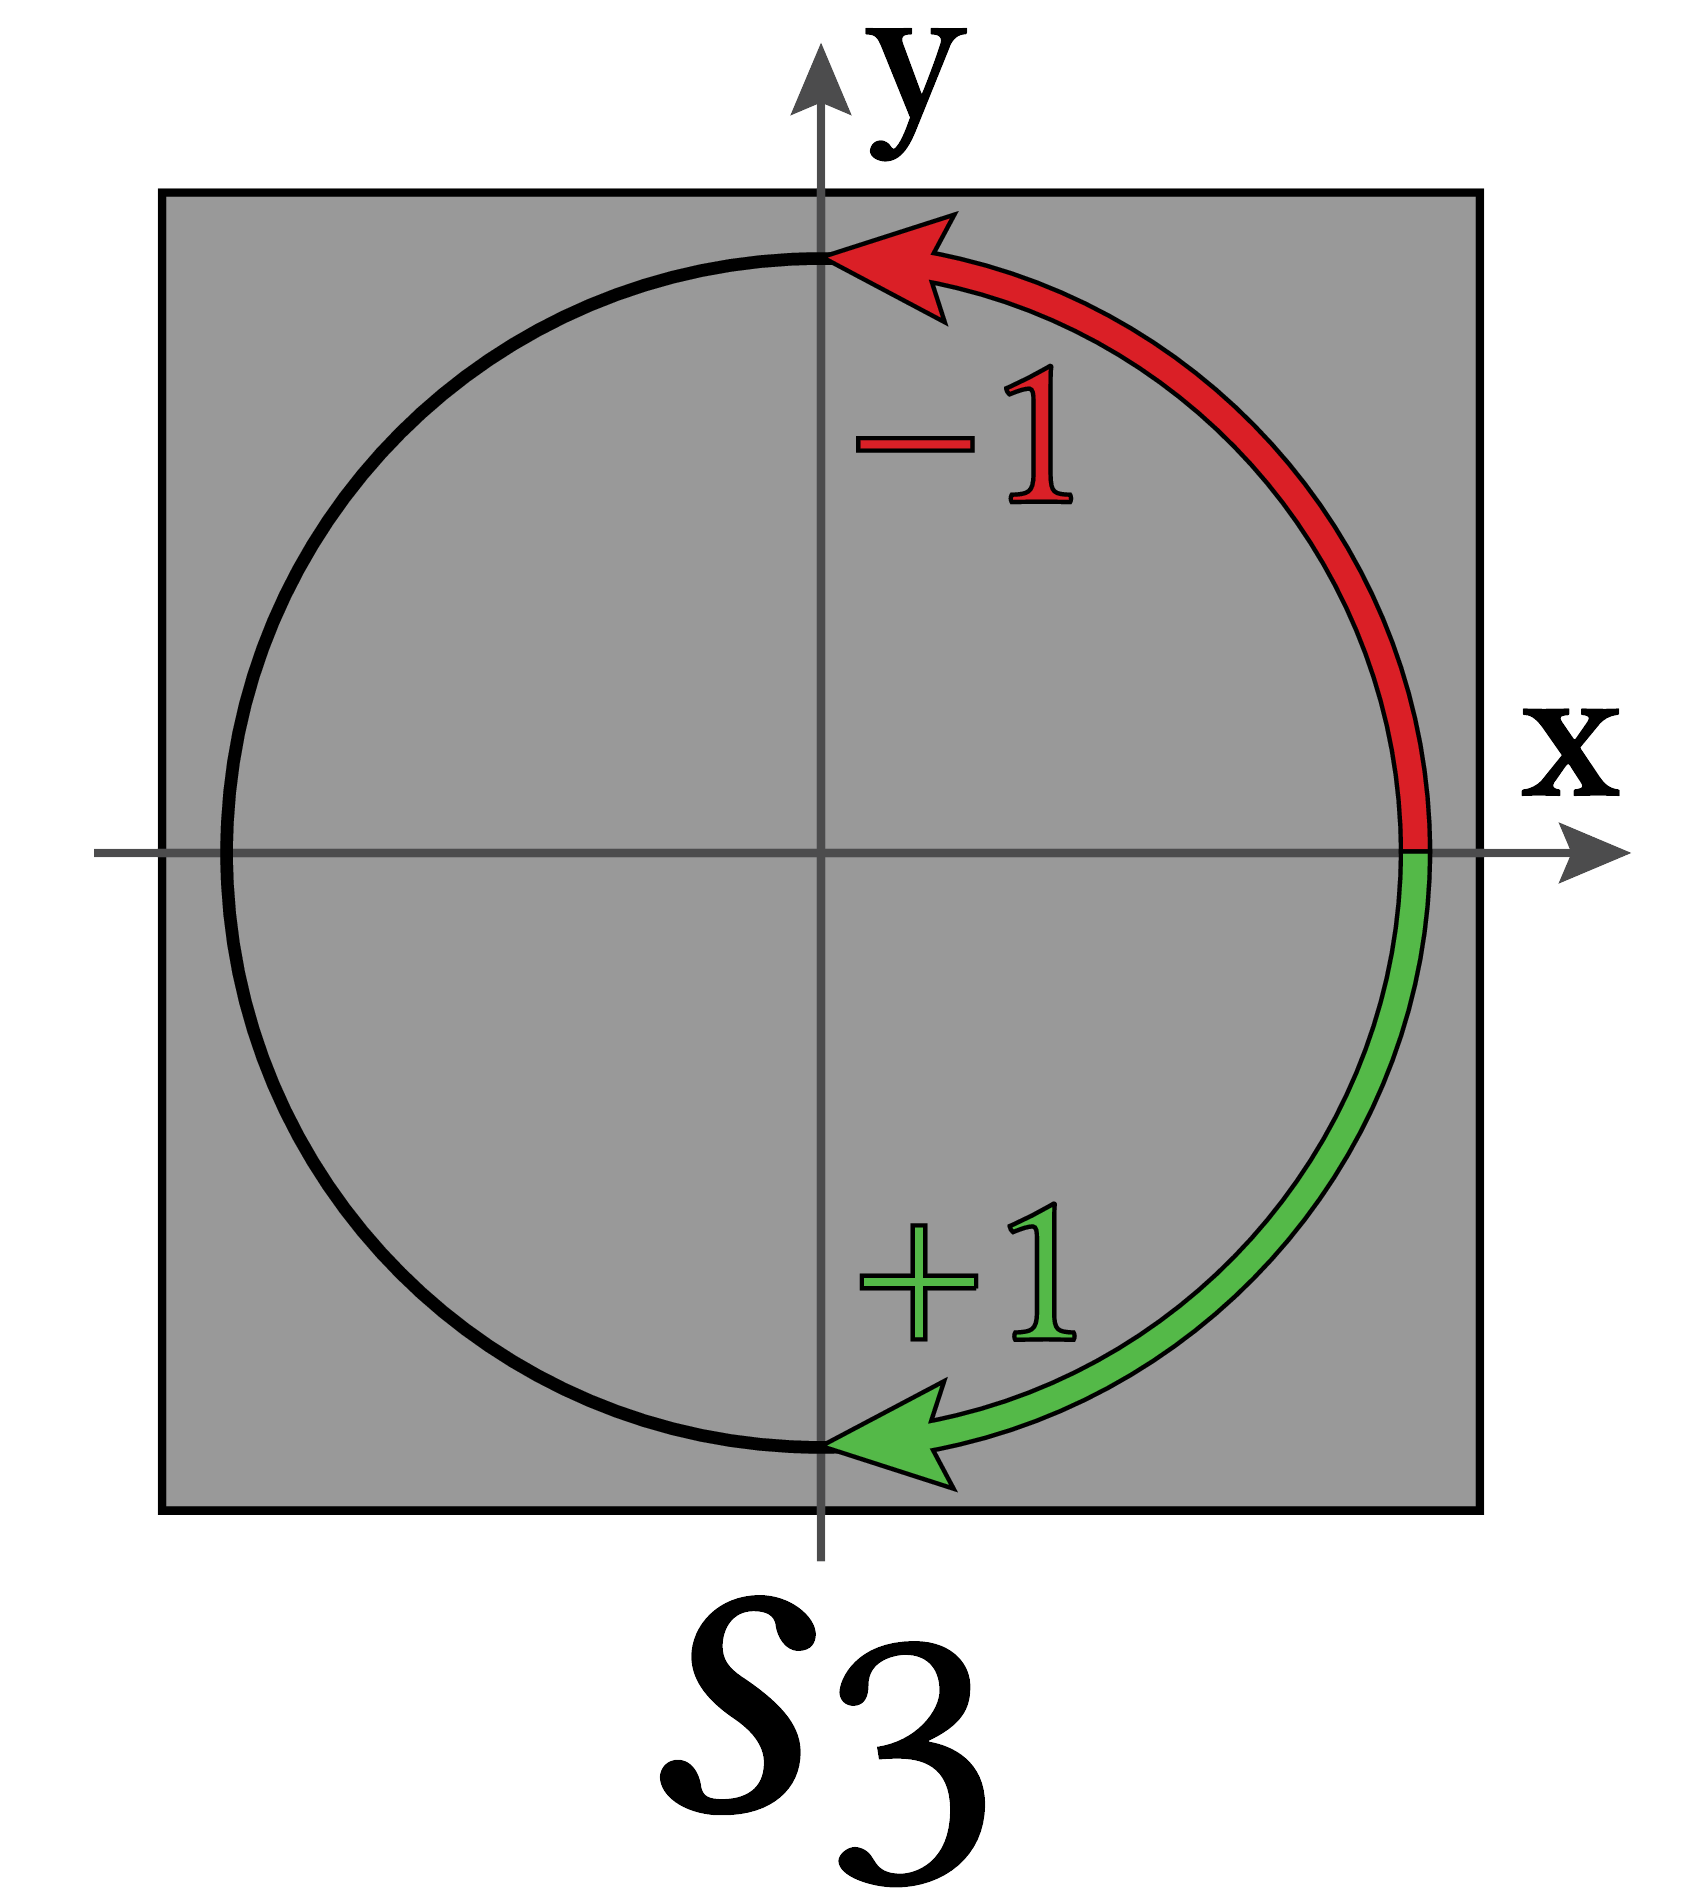
\includegraphics[width=\linewidth]{img/stokes4.png}
			\caption{Left vs. right circular polarization}
		\end{subfigure}
	\end{tabular}
	\caption{Different information carried by the Stokes vector}
	\label{fig:stokes}
\end{figure}

Also, it is necessary to represent the changes to these states upon a surface interaction. A transformation between the incoming state and the outgoing state is represented by the \emph{Mueller matrix} $M \in \R^{4x4}$. Due to the adjustments to all interactions in the light transport, we also generalize the BSDF $f_r(\lambda,\omega_i,\omega_o)$ to the polarized pBSDF $M(\lambda,\omega_i,\omega_o)$.

If the reader is curious about the complications this implementation brings and their solutions, he may want to look into the documentation of Mitsuba2 by \citet{nimier2019mitsuba}. Nevertheless, they are not crucial for the purposes of this thesis and we purposely skip them.

\section{Dispersion}

Generally, the IOR of a dielectric at least slightly varies for different wavelengths (e.g. glass has IOR between 1.5 and 1.6). This causes the polychromatic light to split into its spectral components upon an intersection with such materials. As each wavelength is slightly shifted, a rainbow effect can be perceived --- this phenomenon is called \emph{dispersion}. In nature, it can be frequently seen when light passes through liquids (e.g. sun through the rain). To artificially reproduce spectral dispersion, an object having a shape of a triangular prism, commonly called dispersive prism~\ref{fig:dispersion}, can be used.

\begin{figure}[h]
	\centering
	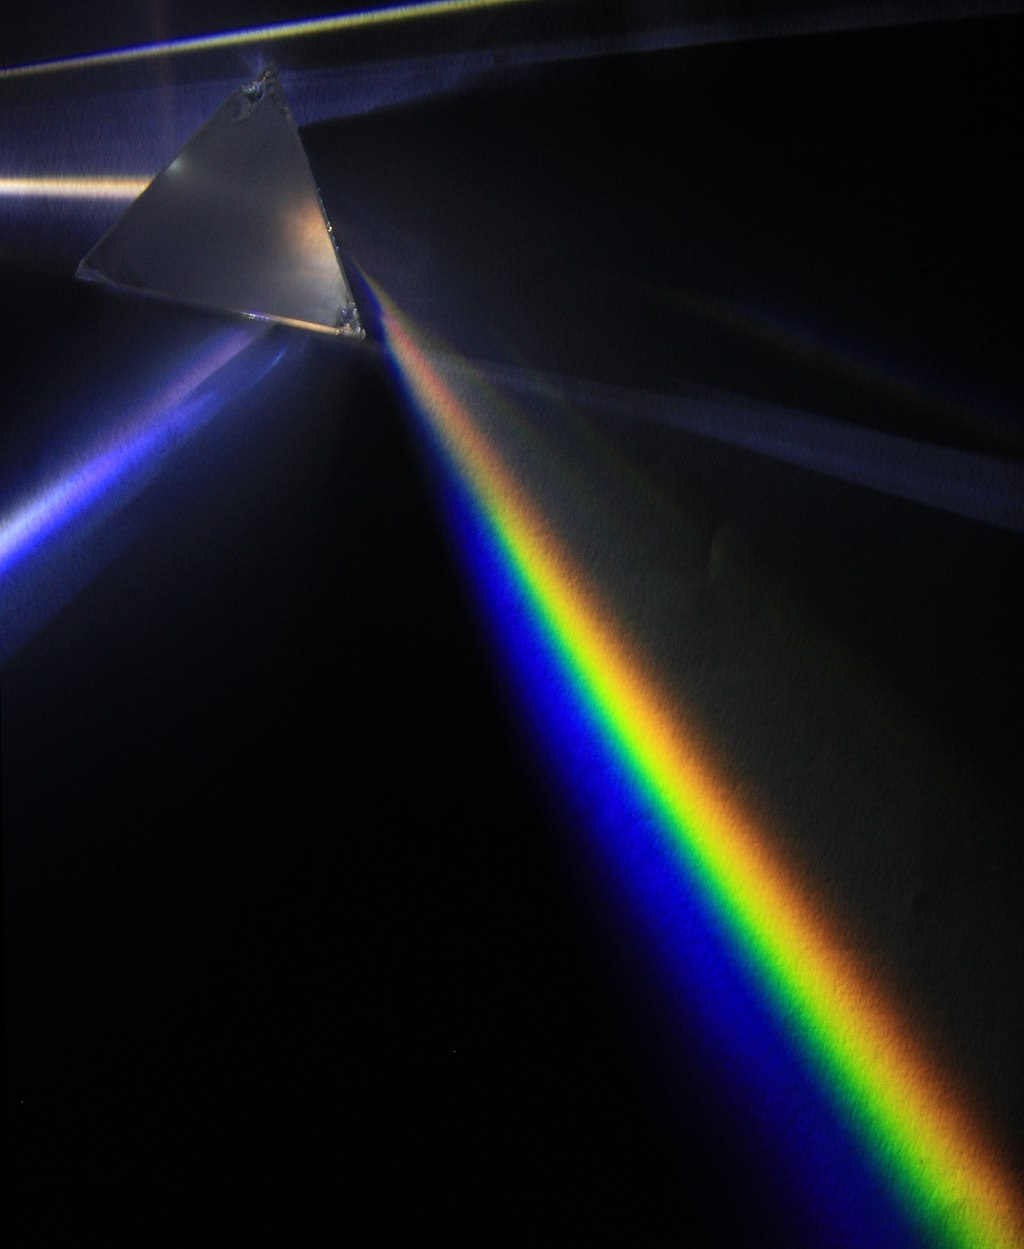
\includegraphics[width=.6\linewidth]{img/dispersion.jpg}
	\caption[nikon]{Photograph of a dispersive prism\footnotemark}
	\label{fig:dispersion}
\end{figure}
\footnotetext{\url{https://en.wikipedia.org/wiki/Dispersive_prism}}


\subsection{Dispersion in rendering}
In computer graphics, even though it is possible to simulate dispersion in the tristimulus rendering, it is insufficient. The obvious choice would be to use spectral rendering, as it already contains most of the information about the tracking of the wavelengths. 

It is necessary to properly represent the varying and not always monotonic IOR --- for these reasons, \emph{Sellmeier approximation}~\cite{wilkie2002tone} is widely used. Then, the renderer must be capable of tracking the possibly dispersed monochromatic rays upon a surface interaction of a single polychromatic ray, i.e. create additional samples that were unnecessary before.

\section{Iridescence}
\label{sec:irid}

It is quite common that some objects in nature exhibit an interesting behavior where the hue of their surface gradually changes with the viewing angle and the illumination angle. This phenomenon is called \emph{iridescence} or \emph{goniochromism} and it can be observed on very thin materials, such as butterfly wings, soap bubbles, oil, etc. It is caused by a large amount of interferences between the light waves and their consequent scattering depending on their wavelength which produces a rapid change in colors~\cite{belcour2017practical}.

We distinguish two main types of iridescence:

\begin{description}
	\item[Microscopic structures] Reflections from structures of a size similar to a light wavelength (e.g. peacock feathers)
	\item[Thin-film] Light interaction with a thin film of a size similar to a light wavelength (e.g. soap bubble)
\end{description}

An example of both can be seen in \autoref{fig:iridescent_example}.

\begin{figure}
	\centering
	\begin{tabular}{cc}
		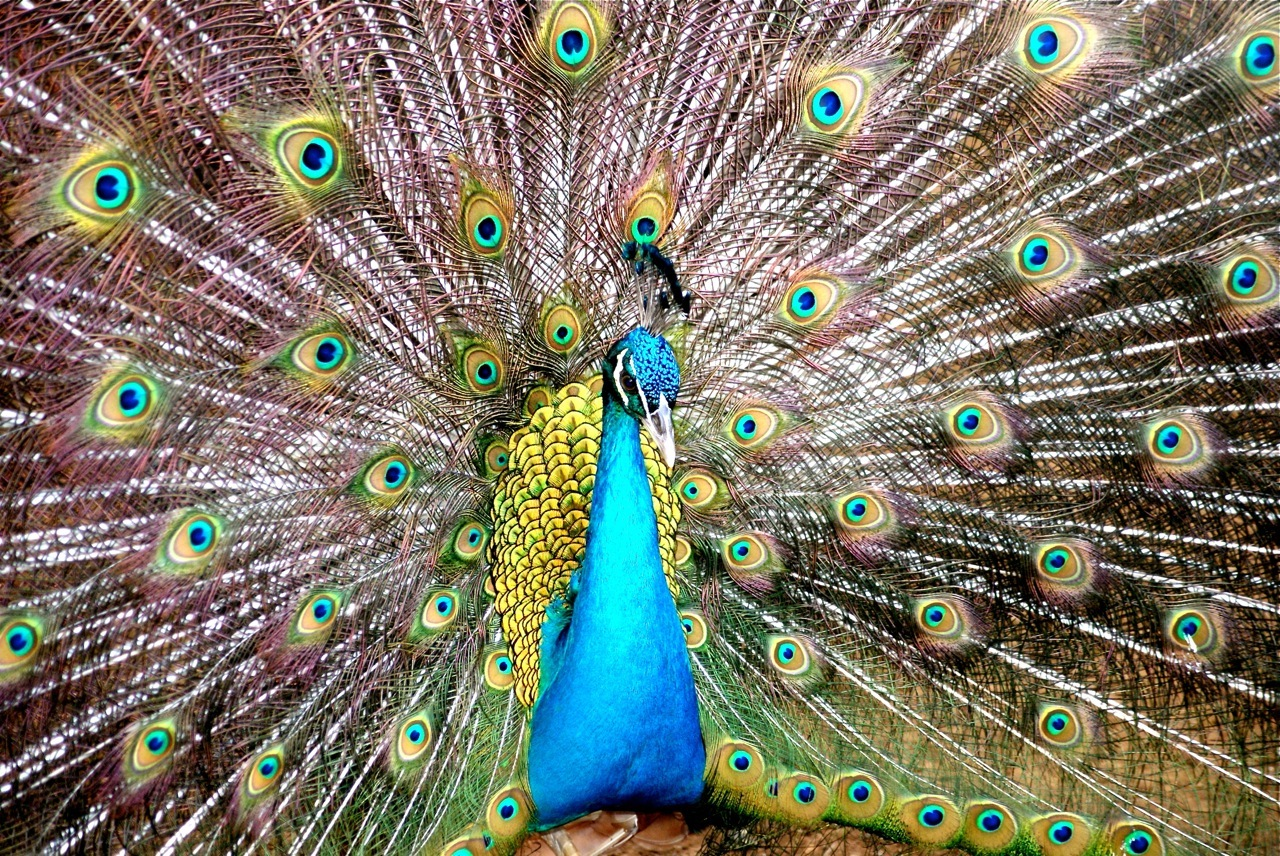
\includegraphics[width=0.4\linewidth]{img/iridescent_peacock.jpg}
		&
		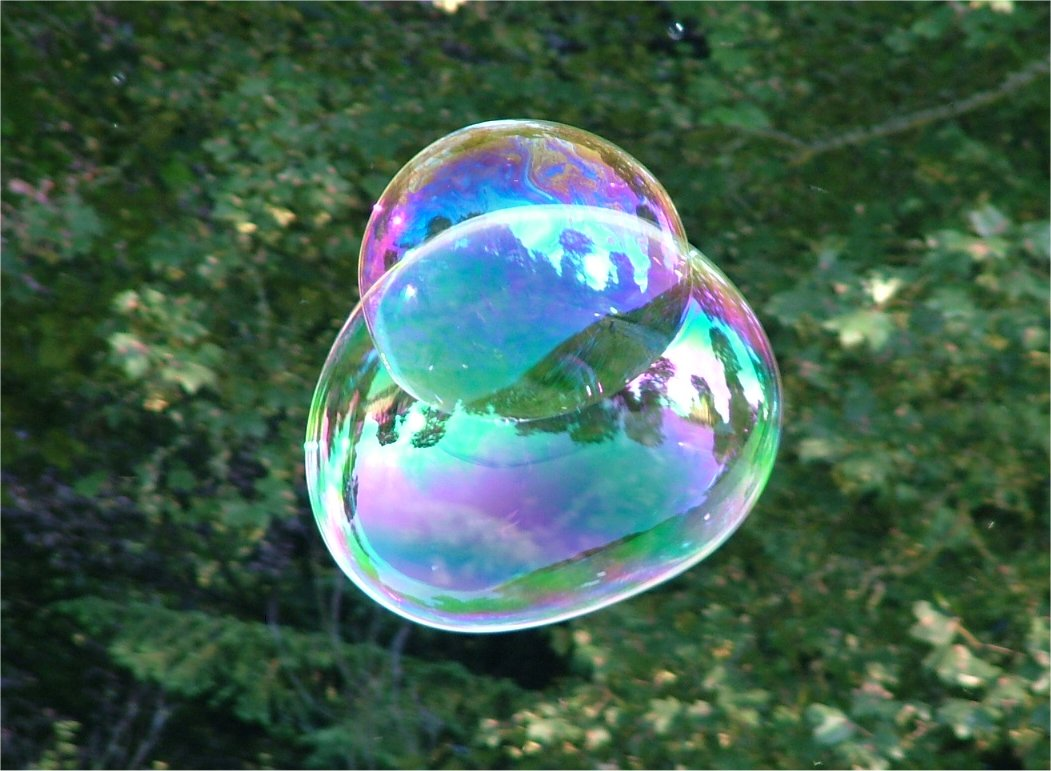
\includegraphics[width=0.4\linewidth]{img/iridescent_soap.jpg}
	\end{tabular}
	\caption[Irid example]{Structural iridescence of peacock feathers (left) and the thin-film light interference in a soap bubble (right)\footnotemark}
	\label{fig:iridescent_example}
\end{figure}
\footnotetext{\url{https://en.wikipedia.org/wiki/Iridescence}}

In this thesis, we focus on the thin-film interference as it is properly described as a physical process and it is already incorporated in Mitsuba~\cite{belcour2017practical}. From now on, by iridescence, we mean the thin-film interference.

First, look at the light interactions inside the membrane of a soap bubble in \autoref{fig:soap}. The light strikes at the surface of the film and, based on the incident angle, it can be either reflected or transmitted. The transmitted light very quickly strikes the bottom boundary of the soap bubble (as it is very thin) and again can be reflected and/or refracted. As the film is a few hundreds of nanometers thick, this repeats with a great frequency and, as you can see, the light transmitted from the upper boundary can easily interfere with the light reflected from the lower boundary.

\begin{figure}[h]
	\centering
	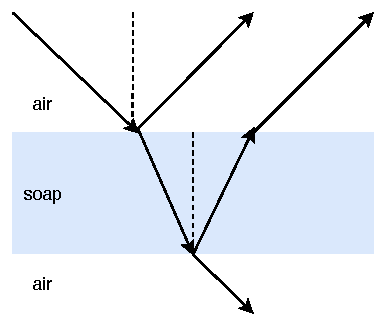
\includegraphics[width=.6\linewidth]{img/soap.pdf}
	\caption{A cross-section of light interactions with a soap bubble}
	\label{fig:soap}
\end{figure}

An obvious observation is that iridescence is also dependent on the thickness of the interacting layer - as the thickness increases, the transmission of the light takes longer time which consequently causes fewer interferences. The difference between two variously thick films is displayed in \autoref{fig:irid_heights}.

\begin{figure}[h]
	\centering
	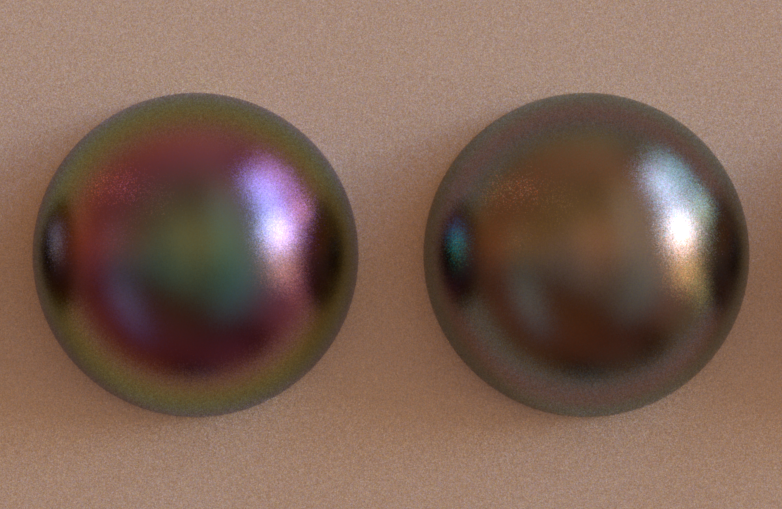
\includegraphics[width=.6\linewidth]{img/irid_heights.png}
	\caption{Two identical rough conductors with differently thick film layers on top of them: 550nm (left) vs. 1500nm (right) rendered in Mitsuba2}
	\label{fig:irid_heights}
\end{figure}

\subsection{Iridescence in rendering}

Based on the publication by \citet{belcour2017practical}, we overview the computational process of iridescence caused by a thin film on top of a rough material. We purposely avoid the exact formulations of the equations, as these would be unnecessarily complicated to explain and it is sufficient to comprehend the basics in order to evaluate the correctness of the computation. For more details, the interested reader is referred to the publication by \citet{belcour2017practical}.

Essentially, the following procedure computes an iridescence term of the thin film layer that is plugged into BSDF of a rough conducting base:

\begin{enumerate}
	\item Compute the reflected and the transmitted values of the Fresnel equations for the IOR of the film and the IOR of the exterior
	\item Compute the optical path differences between the primary and the secondary light paths
	\item Evaluate the Fresnel phase shift
	\item Determine the term by using the Airy summation for the parallel and perpendicular polarization of all consecutive reflections and refractions
\end{enumerate}

\section{Fluorescence}

Curiously, certain materials or substances change their colors with no apparent respect to the illumination color. This behavior is called \emph{fluorescence} and it can be quite commonly observed in nature, e.g. in various minerals but also the living organisms such as fish or arachnids.

The explanation behind this phenomenon is that the molecules of such substances absorb electromagnetic radiation of specific wavelengths and emit back different, usually larger wavelengths. The most eye-catching fluorescence is \\ caused by the absorption of the ultraviolet light which is invisible to the human eye. An example of fluorescent calcite is shown in \autoref{fig:calcite}

\begin{figure}
	\centering
	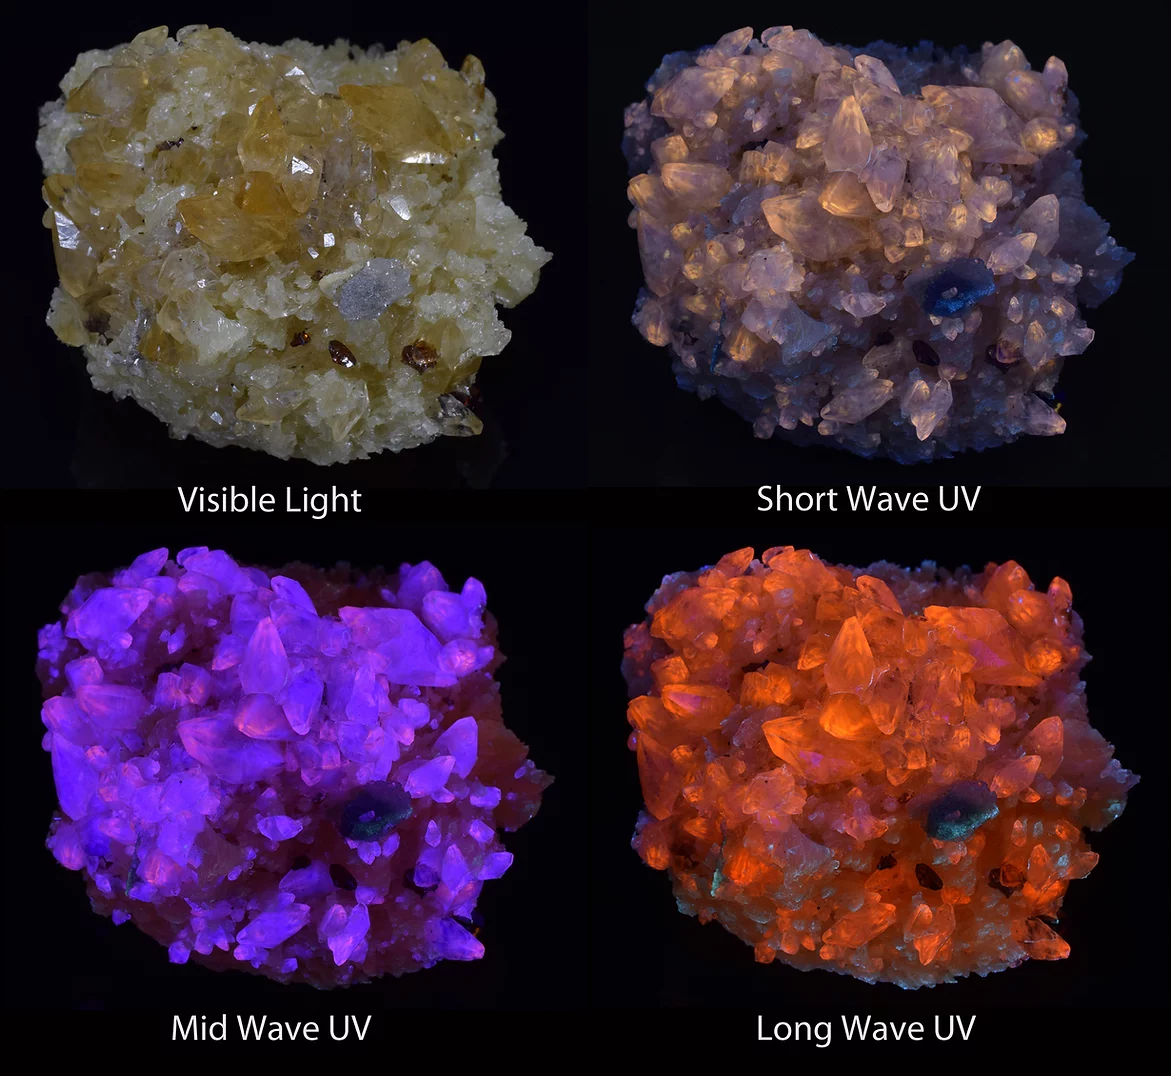
\includegraphics[width=0.8\linewidth]{img/calcite.png}
	\caption[calcite]{Calcite under different lights\footnotemark}
	\label{fig:calcite}
\end{figure}
\footnotetext{\url{https://www.naturesrainbows.com/single-post/2017/11/01/Fluorescent-Multi-Wave-Calcite-from-the-Elmwood-Mine}}

Please note that there is a difference between fluorescence, luminescence and phosphorescence:

\begin{description}
	\item[Luminescence] Natural production of light caused by chemical reactions (no absorption)
	\item[Phosphorescence] Absorbs light and emits different one, even for some time after the light source is gone
	\item[Fluorescence] Absorbs light and emits different one, emission stops almost instantaneously after the light source is gone
\end{description}

\subsection{Fluorescence in rendering}
As we are dealing with the wavelengths of a light spectrum, the appropriate decision is to extend spectral rendering to include fluorescence. Once again, we refer the interested reader to the article by \citet{mojzik2018handling} for the implementation details as, for the purposes of this thesis, we are only covering the fundamental ideas.

As we have mentioned before, we are shifting the wavelengths of the absorbed spectrum to emit a new one --- this is called \emph{Stokes shift} (shown in \autoref{fig:stokes_shift}) and it can be described by \emph{fluorescence response} $\Phi(\lambda_i,\lambda_o)$.

\begin{figure}
	\centering
	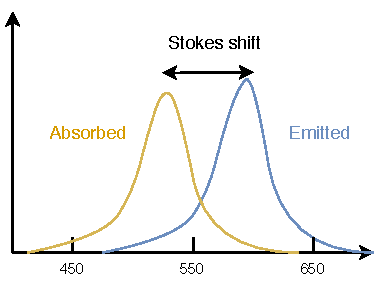
\includegraphics[width=0.7\linewidth]{img/stokes_shift.pdf}
	\caption{Illustration of Stokes shift}
	\label{fig:stokes_shift}
\end{figure}

The discrete form of a fluorescence response can be represented by a \emph{re-radiation matrix}, which contains incoming wavelengths on its vertical axis and their corresponding outgoing wavelengths on its horizontal axis. The probability of the shift follows Kasha's rule --- the spectral distribution of the emitted light should not change, only the intensity of the emission spectrum should.

A generalization of the BRDF that includes re-radiation, called \emph{Bi-spectral Bidirectional Reflectance and Re-radiation distribution function (bi-spectral BRRDF)}, was introduced by \citet{hullin2010acquisition}. It can be denoted by the following equation:

\begin{equation}
f_r((\omega_i,\lambda_i),(\omega_o,\lambda_o))=\frac{d^2L(\omega_o,\lambda_o)}{L(\omega_i,\lambda_i)d\omega_i d\lambda_i}
\end{equation}

The corresponding \emph{bi-spectral rendering equation} can be formulated as follows:
\begin{equation}
L(\omega_o,\lambda_o)=\int_{\Lambda}\int_{\Omega}L(\omega_i,\lambda_i)f_r((\omega_i,\lambda_i),(\omega_o,\lambda_o))d\omega_i d\lambda_i
\end{equation}

Along with polarization, dispersion, iridescence, and reflectance, fluorescence is the last appearance phenomenon that we investigate in this thesis. With all of them covered and properly explained, we may now look into the evaluation process that we propose to determine their accuracy.